\subsection{AddPacketDataCommand}
\begin{sidewaysfigure}
  \centering
  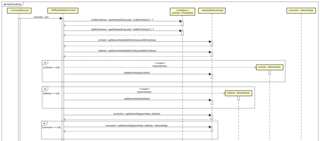
\includegraphics[width=\paperwidth]{../diagramimages/sd_AddPacketData1.png}
  \caption[Sequenzdiagramm AddPacketData]{Sequenzdiagramm AddPacketData}
\end{sidewaysfigure}
\FloatBarrier

\begin{sidewaysfigure}
  \centering
  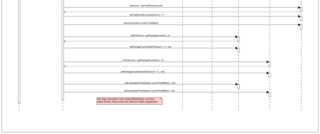
\includegraphics[width=\paperwidth]{../diagramimages/sd_AddPacketData2.png}
  \caption[Sequenzdiagramm AddPacketData]{Sequenzdiagramm AddPacketData}
\end{sidewaysfigure}
\FloatBarrier

Dieses Sequenzdiagramm stellt grob den Ablauf des AddPacketDataCommands (im Folgenden APDC) dar. Jeder APDC prüft zunächst,
ob schon ein Knoten unter der entsprechenden MAC-Addresse vorhanden ist. Falls einer der Knoten (source oder destination)
noch nicht im Graph existiert, wird dieser erstellt und anschließend dem Graph hinzugefügt. Nachdem dies erfolgt ist, wird
geprüft, ob schon eine Verbindung (Kante) zwischen den Knoten besteht, und falls nötig dem Graph hinzugefügt.
Im Anschluss daran werden die einzelnen Knoten- und Kantenstatistiken aktualisiert. Dieser Vorgang ist nur beispielhaft
dargestellt, um das Diagramm nicht zu überladen.
